% Build: cd docs/reports/reconstruction && latexmk -xelatex rk_reconstruction_status_20260416.tex
\documentclass[aspectratio=169]{beamer}
\usetheme{Madrid}
\usecolortheme{default}

\usepackage{amsmath,amssymb}
\usepackage{booktabs}
\usepackage{multirow}
\usepackage{siunitx}
\usepackage{xcolor}
\usepackage{graphicx}
\usepackage{tikz}
\usetikzlibrary{arrows.meta,positioning,calc}

\definecolor{goodgreen}{RGB}{34,139,34}
\definecolor{warnred}{RGB}{200,50,50}

\title[RK Reconstruction \& Error Analysis]{PDC Target-Momentum Reconstruction:\\Algorithm, Physics, and Uncertainty}
\subtitle{Current Status Report --- April 2026}
\author{Baiting Tian}
\institute{RIKEN Nishina Center / DPOL Experiment}
\date{2026-04-16}

\begin{document}

% ============================================================
\begin{frame}
\titlepage
\end{frame}

% ============================================================
\begin{frame}{Outline}
\tableofcontents
\end{frame}

% ============================================================
\section{Physical Setup}
% ============================================================

\begin{frame}{Coordinate frames: lab vs.\ target (beam-as-Z)}
\small
Two right-handed frames are used consistently throughout this report:
\begin{itemize}
  \item \textbf{Lab frame} (Geant4 world): $+z$ along the nominal SAMURAI beamline,
    $+y$ vertical up. PDC hits, field map, RK integration, and the
    internal least-squares fit all live here.
  \item \textbf{Target frame} (``beam-as-Z'', event-generator input):
    $+z$ along the incident beam direction after the $\alpha_\mathrm{tgt}=3^\circ$
    target tilt; differs from lab by $R_y(-\alpha_\mathrm{tgt})$.
    \texttt{truth\_proton\_p4} stays in this frame (\texttt{fMomentum} is never
    rewritten; the forward $R_y(-\alpha)$ only rotates a local copy used for the
    particle gun).
\end{itemize}

\textbf{All truth vs.\ reco comparisons and all plots in this report are in the target frame.}
The reconstruction tools (\texttt{main.cc}, \texttt{analyze\_pdc\_rk\_error.cc})
apply $R_y(+\alpha_\mathrm{tgt})$ at the write stage; the $3\times3$ momentum
covariance is rotated as $\Sigma'=R\Sigma R^\mathrm{T}$ and $px/py/pz$ intervals
are rebuilt as Gaussian fallbacks from the rotated diagonals. $|\vec p|$ is
rotation-invariant and its interval is passed through unchanged.

Prior to 2026-04-19, this rotation was missing and a systematic
$\Delta p_x \approx -p_z\sin\alpha \approx -33$~MeV/$c$ contaminated the residuals
($p_z \approx 627$~MeV/$c$; if $p_z\!\approx\!1$~GeV/$c$ the offset is $-52$~MeV/$c$).
Fisher 68\% coverage on $p_x$ went from $\approx 0.05$ back to $\approx 0.80$ after the fix.
All plots here were regenerated after the fix.
Shared helpers: \texttt{libs/analysis\_pdc\_reco/include/PDCFrameRotation.hh}.
\end{frame}

% ============================================================
\begin{frame}{SAMURAI Spectrometer Geometry}
\small
\begin{columns}[T]
\column{0.55\textwidth}
\textbf{Coordinate system}: beam along $+z$, vertical $y$, horizontal $x$.

\vspace{0.2cm}
\textbf{Key elements}
\begin{itemize}
\item Target at $z \approx -1070\;\mathrm{mm}$ (inside magnet)
\item SAMURAI dipole: $B \approx 1.15\;\mathrm{T}$, center at origin, rotated $30^\circ$ about $y$
\item PDC1 at $z \approx 4000\;\mathrm{mm}$ (after magnet)
\item PDC2 at $z \approx 5000\;\mathrm{mm}$
\item PDC angular tilt: $\theta_\mathrm{PDC} = 57^\circ$
\end{itemize}

\vspace{0.2cm}
\textbf{Typical proton}: $|\vec{p}| \approx 635$ MeV/$c$, $p_z \approx 627$ MeV/$c$.

\column{0.42\textwidth}
\centering
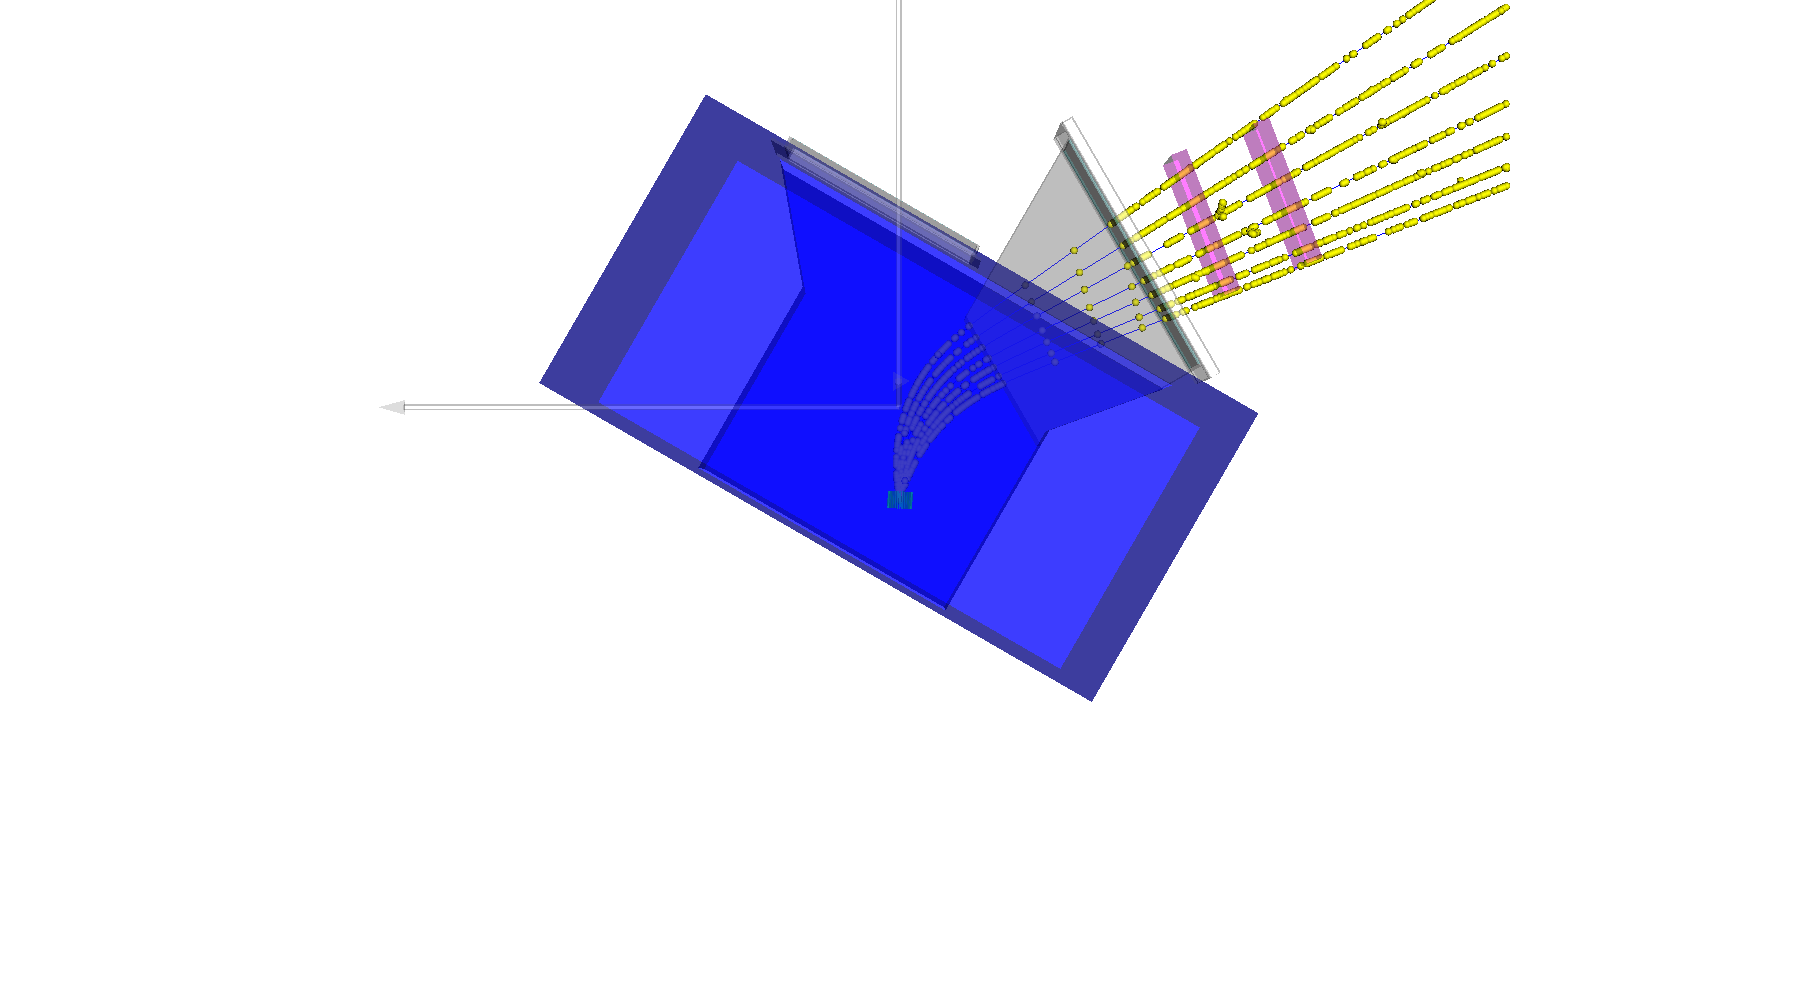
\includegraphics[width=\textwidth]{figures/geometry/samurai_geometry_xz.png}
\vspace{-0.3cm}
{\tiny Geant4 VRML render ($xz$ plane)}
\end{columns}
\end{frame}

% ============================================================
\begin{frame}{PDC Wire Coordinate System}
\small
\textbf{PDC detects two 1D coordinates per plane}: $u$ and $v$.

Given the PDC angular tilt $\theta$ (= $57^\circ$), the lab-frame wire directions are:
\begin{align}
\hat{u} &= \frac{1}{\sqrt{2}}\bigl(\cos\theta,\; +1,\; \sin\theta\bigr), &
\hat{v} &= \frac{1}{\sqrt{2}}\bigl(\cos\theta,\; -1,\; \sin\theta\bigr).
\end{align}

Wire coordinate values from the simulation (\texttt{PDCSimAna}):
\[
u = \frac{x_\mathrm{rot} + y}{\sqrt{2}}, \qquad
v = \frac{-x_\mathrm{rot} + y}{\sqrt{2}},
\]
where $x_\mathrm{rot} = \Delta x \cos\theta - \Delta z \sin\theta$ is the position relative to PDC center, rotated by the PDC tilt angle.

\vspace{0.2cm}
\textbf{Key point}: $\hat{u}$ and $\hat{v}$ have non-zero $z$ components. The $z$-component carries the curvature information from the magnetic deflection. Discarding it (projecting to the $xy$-plane) destroys the momentum sensitivity.
\end{frame}

% ============================================================
\section{RK Trajectory Model}
% ============================================================

\begin{frame}{Relativistic Equation of Motion}
\small
A charged particle with charge $q$, momentum $\vec{p}$, and energy $E = \sqrt{|\vec{p}|^2 + m^2}$ in a magnetic field $\vec{B}(\vec{r})$ obeys:
\begin{align}
\frac{d\vec{r}}{dt} &= \frac{\vec{p}\,c^2}{E} = \vec{v}, \\[4pt]
\frac{d\vec{p}}{dt} &= q\,\vec{v} \times \vec{B}(\vec{r}).
\end{align}

\textbf{Properties}:
\begin{itemize}
\item The Lorentz force is perpendicular to $\vec{v}$, so $|\vec{p}|$ is conserved (no $dE/dx$ in current model).
\item In the rotated SAMURAI field ($B_y$-dominated), the primary bending occurs in the $xz$-plane.
\end{itemize}

\vspace{0.2cm}
\textbf{Unit system}: positions in mm, time in ns, momenta in MeV/$c$, fields in T.\\
Conversion constant: $q_e \cdot c = 89.876\;\mathrm{MeV/(c \cdot T \cdot ns)}$.
\end{frame}

% ============================================================
\begin{frame}{4th-Order Runge-Kutta Integration (RK4)}
\small
State vector $\vec{Y} = (\vec{r},\, \vec{p})$ is evolved with fixed step $\Delta t$:
\begin{align*}
\vec{K}_1 &= f\bigl(\vec{Y}_n\bigr), \\
\vec{K}_2 &= f\bigl(\vec{Y}_n + \tfrac{\Delta t}{2}\vec{K}_1\bigr), \\
\vec{K}_3 &= f\bigl(\vec{Y}_n + \tfrac{\Delta t}{2}\vec{K}_2\bigr), \\
\vec{K}_4 &= f\bigl(\vec{Y}_n + \Delta t\,\vec{K}_3\bigr), \\[4pt]
\vec{Y}_{n+1} &= \vec{Y}_n + \frac{\Delta t}{6}\bigl(\vec{K}_1 + 2\vec{K}_2 + 2\vec{K}_3 + \vec{K}_4\bigr),
\end{align*}
where $f(\vec{r}, \vec{p}) = \bigl(\vec{p}\,c^2/E,\; q\,\vec{v}\times\vec{B}(\vec{r})\bigr)$.

\vspace{0.2cm}
Each step queries the field map $\vec{B}(\vec{r})$ four times. The trajectory is stored as a sequence of $(\vec{r}_i, \vec{p}_i, t_i)$ points.

\vspace{0.2cm}
\textbf{Default step}: $\Delta t \sim 0.1$ ns ($\approx 30$ mm spatial step), $\sim$150--200 steps from target to PDC2.
\end{frame}

% ============================================================
\section{Least-Squares Fitting}
% ============================================================

\begin{frame}{Parameterization}
\small
\textbf{State vector} (5 parameters):
\[
\vec{\alpha} = \bigl(\delta x,\; \delta y,\; u,\; v,\; p\bigr),
\]
where:
\begin{itemize}
\item $\delta x$, $\delta y$ --- target position offset from nominal [mm]
\item $u = p_x / p_z$, $v = p_y / p_z$ --- direction tangents at the target
\item $p = |\vec{p}|$ --- total momentum magnitude [MeV/$c$]
\end{itemize}

Momentum vector reconstructed as:
\[
p_z = \frac{p}{\sqrt{1 + u^2 + v^2}}, \qquad
p_x = u \cdot p_z, \qquad
p_y = v \cdot p_z.
\]

\vspace{0.1cm}
\textbf{Fit modes}:
\begin{itemize}
\item \texttt{kFixedTargetPdcOnly}: 3 free params $(u, v, p)$, $\delta x = \delta y = 0$ (fixed target)
\item \texttt{kThreePointFree}: 5 free params $(\delta x, \delta y, u, v, p)$ with soft target prior
\end{itemize}
\end{frame}

% ============================================================
\begin{frame}{Residual Construction}
\small
For each PDC plane $k \in \{1,2\}$, the trajectory point closest to the measured hit $\vec{r}_k^\mathrm{meas}$ is found. The 3D displacement is projected onto the wire directions:
\begin{align}
r_u^{(k)} &= \bigl(\vec{r}_k^\mathrm{traj} - \vec{r}_k^\mathrm{meas}\bigr) \cdot \hat{u}, &
r_v^{(k)} &= \bigl(\vec{r}_k^\mathrm{traj} - \vec{r}_k^\mathrm{meas}\bigr) \cdot \hat{v}.
\end{align}

These raw residuals are \textbf{whitened} via a 2$\times$2 Cholesky decomposition of the measurement covariance:
\[
C = \begin{pmatrix} \sigma_u^2 & \rho\,\sigma_u\sigma_v \\ \rho\,\sigma_u\sigma_v & \sigma_v^2 \end{pmatrix},
\qquad
\begin{pmatrix} w_1 \\ w_2 \end{pmatrix}
= L^{-1}
\begin{pmatrix} r_u \\ r_v \end{pmatrix},
\quad C = L L^T.
\]

After whitening, each $w_i \sim \mathcal{N}(0, 1)$ is an independent, unit-variance residual.

\vspace{0.1cm}
\textbf{Total}: 4 residuals (2 per plane). In \texttt{kThreePointFree} mode, 2 additional target-constraint residuals: $w_5 = \delta x / \sigma_\mathrm{tgt}$, $w_6 = \delta y / \sigma_\mathrm{tgt}$.
\end{frame}

% ============================================================
\begin{frame}{$\chi^2$ and Degrees of Freedom}
\small
\[
\chi^2(\vec{\alpha}) = \sum_{i=1}^{N_\mathrm{res}} w_i^2(\vec{\alpha})
\]

\begin{table}
\centering
\begin{tabular}{lccccc}
\toprule
Mode & Free params & PDC residuals & Target residuals & $N_\mathrm{res}$ & $N_\mathrm{dof}$ \\
\midrule
\texttt{kFixedTargetPdcOnly} & $u, v, p$ & 4 & 0 & 4 & 1 \\
\texttt{kThreePointFree} & $\delta x, \delta y, u, v, p$ & 4 & 2 & 6 & 1 \\
\bottomrule
\end{tabular}
\end{table}

\vspace{0.2cm}
The Jacobian $J_{ij} = \partial w_i / \partial \alpha_j$ is computed by central finite differences (each column requires two additional RK trajectory evaluations).
\end{frame}

% ============================================================
\begin{frame}{Levenberg-Marquardt Optimization}
\small
At each iteration, the normal equation is solved:
\[
\bigl(J^T J + \lambda \cdot \mathrm{diag}(J^T J)\bigr)\,\Delta\vec{\alpha} = -J^T \vec{w},
\]
where $\lambda$ is the damping parameter.

\textbf{Update rules}:
\begin{itemize}
\item If $\chi^2_\mathrm{new} < \chi^2_\mathrm{old}$: accept step, $\lambda \to \lambda / 3$
\item Otherwise: reject step, $\lambda \to 4\lambda$
\end{itemize}

\textbf{Convergence}: $\Delta\chi^2 < 10^{-8}$ or $\|\Delta\vec{\alpha}\| < 10^{-5}$.

\vspace{0.2cm}
\textbf{Initialization challenge}: the straight-line direction from target to PDC is off by $\sim\!25^\circ$ due to magnetic bending. Without a good starting point, LM converges to wrong local minima.
\end{frame}

% ============================================================
\begin{frame}{Coarse Grid Search + Multi-Start Strategy}
\small
\textbf{Problem}: single initial guess leads to convergence failures for many momentum values.

\textbf{Solution}: two-phase initialization.

\vspace{0.1cm}
\textbf{Phase 1: Grid search} over $N_u \times N_v \times N_p = 7 \times 3 \times 5 = 105$ candidate states:
\begin{itemize}
\item $u \in [u_\mathrm{line} - 1.0,\; u_\mathrm{line} + 1.0]$ (7 points, accounts for $\pm 45^\circ$ deflection)
\item $v \in [v_\mathrm{line} - 0.3,\; v_\mathrm{line} + 0.3]$ (3 points, less out-of-plane bending)
\item $p \in \{200, 400, 700, 1200, 2000\}$ MeV/$c$
\end{itemize}
Each candidate is evaluated once ($\sim\!0.1$ ms per \texttt{Evaluate}). Total: $\sim\!10$ ms.

\vspace{0.1cm}
\textbf{Phase 2: Multi-start LM} from the 5 lowest-$\chi^2$ grid candidates. The LM result with the global-minimum $\chi^2$ is selected.

Cost: $5 \times$ LM convergence $\approx 50$ ms. Fully acceptable for offline reconstruction.
\end{frame}

% ============================================================
\section{Uncertainty Estimation}
% ============================================================

\begin{frame}{Overview of Error Analysis Methods}
\small
\begin{table}
\centering
\begin{tabular}{p{0.15\textwidth}p{0.30\textwidth}p{0.22\textwidth}p{0.22\textwidth}}
\toprule
Method & Construction & Meaning & Cost \\
\midrule
\textbf{Fisher} & $\Sigma = (J^TJ)^{-1}$ at MLE & Local Gaussian $\approx$ of likelihood & 1 Jacobian \\
\textbf{Profile LH} & Scan one $\alpha_k$, minimize others; $\Delta\chi^2 = 1$ crossings & Frequentist CI & $\sim\!20$ LM per param \\
\textbf{Laplace} & $(J^TJ + \Lambda_\mathrm{prior})^{-1}$ at MAP & Bayesian credible interval (Gaussian $\approx$) & 1 matrix inversion \\
\textbf{MCMC} & Metropolis-Hastings random walk in $\vec{\alpha}$ space & Full Bayesian posterior & $\sim\!50$k steps \\
\textbf{MC Prop.} & 256 Gaussian samples in $(u,v,p)$, transform to $(p_x,p_y,p_z)$ & Nonlinear error propagation & 256 transforms \\
\bottomrule
\end{tabular}
\end{table}

\vspace{0.1cm}
Fisher and Laplace are fast (every event); Profile LH and MCMC are offline diagnostics.\\
MC propagation captures nonlinear asymmetry in the $(u,v,p) \to (p_x,p_y,p_z)$ mapping.
\end{frame}

% ============================================================
\begin{frame}{Fisher Information}
\small
At the MLE $\hat{\vec{\alpha}}$, the observed Fisher information matrix is:
\[
\mathcal{I}(\hat{\vec{\alpha}}) = J^T J,
\]
where $J_{ij} = \partial w_i / \partial \alpha_j$ is the whitened-residual Jacobian.

The parameter covariance (Cram\'{e}r-Rao bound) is:
\[
\Sigma_{\vec{\alpha}} = \mathcal{I}^{-1} = (J^T J)^{-1}.
\]

Momentum covariance is propagated via the momentum Jacobian $M_{ij} = \partial p_i / \partial \alpha_j$:
\[
\Sigma_{\vec{p}} = M \, \Sigma_{\vec{\alpha}} \, M^T.
\]

Fisher confidence intervals (assuming Gaussian):
\[
p_i \pm z_\alpha \cdot \sqrt{(\Sigma_{\vec{p}})_{ii}}, \qquad z_{0.68} \approx 1.0,\quad z_{0.95} \approx 1.96.
\]
\end{frame}

% ============================================================
\begin{frame}{Monte Carlo Nonlinear Error Propagation}
\small
The transformation $(u, v, p) \to (p_x, p_y, p_z)$ is nonlinear:
\[
p_z = \frac{p}{\sqrt{1 + u^2 + v^2}}, \quad p_x = u \cdot p_z, \quad p_y = v \cdot p_z.
\]

\textbf{Procedure}:
\begin{enumerate}
\item From Fisher covariance $\Sigma_{\vec{\alpha}}$, generate $N = 256$ samples: $\vec{\alpha}^{(k)} \sim \mathcal{N}(\hat{\vec{\alpha}},\, \Sigma_{\vec{\alpha}})$.
\item Transform each sample to momentum space: $\vec{p}^{(k)} = \vec{p}(\vec{\alpha}^{(k)})$.
\item Compute empirical percentiles:
\begin{itemize}
\item 68\% interval: $[q_{16},\; q_{84}]$
\item 95\% interval: $[q_{2.5},\; q_{97.5}]$
\end{itemize}
\end{enumerate}

\textbf{Advantages}:
\begin{itemize}
\item Captures asymmetric intervals automatically.
\item No linearization (delta method) assumption needed.
\item Cheap: only 256 algebraic transforms, no RK trajectory evaluations.
\end{itemize}
\end{frame}

% ============================================================
\begin{frame}{Profile Likelihood}
\small
For each active parameter $\alpha_k$, scan a grid of values while minimizing $\chi^2$ over the remaining parameters:
\[
\chi^2_\mathrm{profile}(\alpha_k) = \min_{\alpha_{j \neq k}} \chi^2(\vec{\alpha}).
\]

The confidence interval is defined by:
\[
\Delta\chi^2 = \chi^2_\mathrm{profile}(\alpha_k) - \chi^2_\mathrm{min} \leq \Delta\chi^2_\mathrm{crit},
\]
where $\Delta\chi^2_\mathrm{crit} = 1.0$ for 68\% CL and $4.0$ for 95\% CL (1 parameter of interest).

\vspace{0.2cm}
\textbf{Implementation}: warm-start LM (previous scan point provides the initial guess for the next), linear interpolation for crossing detection.

\vspace{0.2cm}
\textbf{Use case}: diagnose non-Gaussian/asymmetric likelihood structure. Especially important for $p$ near the boundary ($p_\mathrm{min}$ or $p_\mathrm{max}$).
\end{frame}

% ============================================================
\begin{frame}{Bayesian Posterior (Laplace + MCMC)}
\small
\textbf{Posterior}:
\[
\log \pi(\vec{\alpha} \mid \mathrm{data}) \propto -\tfrac{1}{2}\chi^2(\vec{\alpha}) + \log \pi_0(\vec{\alpha}),
\]
where the prior $\pi_0$ is flat on $(u, v, \delta x, \delta y)$ and optionally Gaussian on $p$:
\[
\log \pi_0(p) = -\frac{(p - p_0)^2}{2\sigma_p^2}.
\]

\textbf{Laplace approximation}: Gaussian around MAP with covariance $(J^TJ + \Lambda_\mathrm{prior})^{-1}$.

\vspace{0.1cm}
\textbf{MCMC}: Metropolis-Hastings with adaptive proposal:
\begin{itemize}
\item Proposal: $\vec{\alpha}' = \vec{\alpha} + s \cdot L \cdot \vec{z}$, \quad $\vec{z} \sim \mathcal{N}(0, I)$, \quad $LL^T = \Sigma_\mathrm{posterior}$
\item Acceptance: $\min\bigl(1,\, \exp(\Delta \log\pi)\bigr)$
\item Adaptive scale $s$: adjusted during burn-in to target 23\% acceptance rate
\item Burn-in: 5000 steps; post-burn: 50000 steps, thin every 5
\item Diagnostics: Geweke $z$-score (stationarity), effective sample size (autocorrelation)
\end{itemize}
\end{frame}

% ============================================================
\section{Current Performance}
% ============================================================

\begin{frame}{E2E Test Results: RK vs NN}
\small
\textbf{Test setup}: Geant4 simulation $\to$ PDC reconstruction $\to$ target momentum reconstruction $\to$ truth comparison. 5 truth grid points, $p_z = 627$ MeV/$c$, 1 event each.

\begin{table}
\centering
\begin{tabular}{rrrrrrrr}
\toprule
$p_x^\mathrm{true}$ & \multicolumn{3}{c}{RK bias (MeV/$c$)} & \multicolumn{3}{c}{NN bias (MeV/$c$)} \\
\cmidrule(lr){2-4} \cmidrule(lr){5-7}
(MeV/$c$) & $\Delta p_x$ & $\Delta p_y$ & $\Delta p_z$ & $\Delta p_x$ & $\Delta p_y$ & $\Delta p_z$ \\
\midrule
$-100$ & $-7.3$ & $-13.4$ & $-16.1$ & $-6.2$ & $-13.0$ & $-5.4$ \\
$-50$ & $-20.4$ & $-25.5$ & $-10.8$ & $-20.5$ & $-24.9$ & $-0.7$ \\
$0$ & $3.3$ & $-3.9$ & $-13.1$ & $3.5$ & $-3.8$ & $-3.0$ \\
$+50$ & $-33.3$ & $16.3$ & $-8.7$ & $-31.4$ & $16.8$ & $-0.2$ \\
$+100$ & $-37.8$ & $-20.9$ & $-5.3$ & $-43.6$ & $-19.4$ & $6.3$ \\
\bottomrule
\end{tabular}
\end{table}

\begin{itemize}
\item $p_x$/$p_y$ biases are comparable between RK and NN (dominated by single-event Geant4 fluctuations).
\item $p_z$: RK shows a systematic negative bias ($-5$ to $-16$ MeV/$c$), likely from missing $dE/dx$.
\end{itemize}
\end{frame}

% ============================================================
\begin{frame}{Three RK Modes --- Unified Performance}
\small
All three modes now use the same \texttt{RkLeastSquaresAnalyzer} with correct wire-coordinate residuals and multi-start initialization.

\begin{table}
\centering
\begin{tabular}{lrrr}
\toprule
Mode & Mean $|\mathrm{bias}_{p_x}|$ & Mean $|\mathrm{bias}_{p_y}|$ & Mean $|\mathrm{bias}_{p_z}|$ \\
 & (MeV/$c$) & (MeV/$c$) & (MeV/$c$) \\
\midrule
\texttt{kFixedTargetPdcOnly} & 20.4 & 16.0 & 10.8 \\
\texttt{kTwoPointBackprop} & 20.4 & 16.0 & 10.8 \\
\texttt{kThreePointFree} & 21.3 & 16.2 & 10.3 \\
\midrule
NN (reference) & 21.0 & 15.6 & 3.1 \\
\bottomrule
\end{tabular}
\end{table}

\vspace{0.2cm}
\textbf{Before the bug fixes}, the RK modes had mean biases of 180--650 MeV/$c$ on $p_x$ and 190--605 MeV/$c$ on $p_z$. The improvement is $\mathbf{10\text{--}80\times}$.
\end{frame}

% ============================================================
\section{Theoretical Resolution Limits}
% ============================================================

\begin{frame}{Cram\'{e}r-Rao Bound from Spectrometer Geometry}
\small
\textbf{Bending radius and deflection}:
\[
B\rho = \frac{p}{0.3\,q} = \frac{635}{300} = 2.12\;\mathrm{T{\cdot}m}, \quad
\rho = \frac{B\rho}{B} = \frac{2.12}{1.15} = 1840\;\mathrm{mm},
\]
\[
\theta_\mathrm{bend} \approx \frac{L_\mathrm{eff}}{\rho} = \frac{800}{1840} \approx 0.43\;\mathrm{rad} \approx 25^\circ.
\]

\textbf{Momentum resolution} from two-point exit angle measurement:
\[
\sigma_\theta = \frac{\sigma_x \sqrt{2}}{L_{12}}, \qquad
\sigma_p = \frac{\sigma_\theta}{\bigl|\partial\theta_\mathrm{bend}/\partial p\bigr|}
= \frac{p}{\theta_\mathrm{bend}} \cdot \sigma_\theta.
\]

\begin{table}
\centering
\begin{tabular}{lccc}
\toprule
$\sigma_x$ & $\sigma_\theta$ (mrad) & $\sigma_p$ (MeV/$c$) & Note \\
\midrule
0.5 mm & 0.71 & 1.0 & Geant4 smearing \\
2.0 mm & 2.83 & 4.1 & Fitter setting \\
\bottomrule
\end{tabular}
\end{table}

This is the \emph{position-only} limit assuming no multiple scattering.
\end{frame}

% ============================================================
\begin{frame}{Multiple Scattering: Highland Formula}
\small
For a 635~MeV/$c$ proton ($\beta = 0.560$, $\beta p = 356$~MeV/$c$):
\[
\theta_0 = \frac{13.6\;\mathrm{MeV}}{\beta p}\;\sqrt{\frac{x}{X_0}}\;
\Bigl[1 + 0.038\,\ln\!\bigl(x/X_0\bigr)\Bigr].
\]

\begin{table}
\centering
\begin{tabular}{lcccc}
\toprule
Material & Thickness & $X_0$ (g/cm$^2$) & $x/X_0$ & $\theta_0$ (mrad) \\
\midrule
Sn target & 2.5~mm (avg) & 8.82 & 0.207 & 16.4 \\
Air (1~atm) & 1~m & 36.66 & $3.29{\times}10^{-3}$ & 1.72 \\
PDC gas$^\dagger$ & 224~mm & 24.1 & $1.74{\times}10^{-3}$ & 1.21 \\
\bottomrule
\end{tabular}
\end{table}
{\footnotesize $^\dagger$75\% Ar + 25\% i-C$_4$H$_{10}$ at 1~atm; effective path at $32^\circ$ incidence; per PDC.}

\vspace{0.15cm}
\textbf{Target} (16.4~mrad): absorbed by direction fit parameters $(u,v)$; negligible effect on $|\vec{p}|$.

\textbf{Air + PDC gas}: scattering \emph{after} the field corrupts the exit angle measurement.
\end{frame}

% ============================================================
\begin{frame}{Combined Resolution Estimate}
\small
MS corrupts the exit angle by $\sigma_{\theta,\mathrm{MS}} = \sqrt{\theta_{0,\mathrm{air}}^2 + \theta_{0,\mathrm{PDC1}}^2} = \sqrt{1.72^2 + 1.21^2} = 2.10$~mrad.

Using $\sigma_p = (p / \theta_\mathrm{bend})\,\sigma_\theta$:

\begin{table}
\centering
\begin{tabular}{lcc}
\toprule
Source & $\sigma_\theta$ (mrad) & $\sigma_p$ (MeV/$c$) \\
\midrule
Position ($\sigma_x{=}0.5$~mm) & 0.71 & 1.0 \\
MS: Air (1~m) & 1.72 & 2.5 \\
MS: PDC1 gas & 1.21 & 1.8 \\
\midrule
\textbf{Combined} ($\sigma_x{=}0.5$~mm) & \textbf{2.22} & \textbf{3.2} \\
\textbf{Combined} ($\sigma_x{=}2.0$~mm) & \textbf{3.52} & \textbf{5.1} \\
\bottomrule
\end{tabular}
\end{table}

\begin{table}
\centering
\begin{tabular}{lccc}
\toprule
 & Theory ($\sigma_x{=}0.5$) & NN MAE ($p_z$) & RK MAE ($p_z$) \\
\midrule
$p_z$ & 3.2 MeV/$c$ & 3.1 MeV/$c$ & 10.8 MeV/$c$ \\
\bottomrule
\end{tabular}
\end{table}

{\footnotesize NN/RK MAE from \texttt{test\_rk\_nn\_comparison.py} on 5 E2E grid events. RK $p_z$ bias ($-10.8$~MeV/$c$ mean) attributed to missing $dE/dx$.}
\end{frame}

% ============================================================
\begin{frame}{Error Analysis Results (from \texttt{analyze\_pdc\_rk\_error})}
\small
\textbf{All numbers from actual test output} --- \texttt{build/test\_output/error\_analysis\_rk/}.

\begin{table}
\centering
\begin{tabular}{rcccc}
\toprule
Event & $\sigma_{p_x}^\mathrm{Fish}$ & $\sigma_{p_y}^\mathrm{Fish}$ & $\sigma_{p_z}^\mathrm{Fish}$ & $\chi^2_\mathrm{red}$ \\
 & (MeV/$c$) & (MeV/$c$) & (MeV/$c$) & \\
\midrule
0 & 3.83 & 0.15 & 2.22 & 0.178 \\
1 & 3.20 & 0.16 & 2.05 & 1.896 \\
2 & 6.50 & 0.15 & 5.41 & 0.613 \\
3 & 6.48 & 0.15 & 5.64 & 0.065 \\
4 & 6.96 & 0.20 & 6.80 & 0.696 \\
\bottomrule
\end{tabular}
\end{table}

\begin{table}
\centering
\begin{tabular}{lc}
\toprule
Metric & Value (MeV/$c$) \\
\midrule
Median Fisher $|\vec{p}|$ width (68\%) & 10.72 \\
Median Profile $|\vec{p}|$ width (68\%) & 10.42 \\
Median MCMC $|\vec{p}|$ width (68\%) & 11.33 \\
Median MCMC acceptance rate & 0.51 \\
\bottomrule
\end{tabular}
\end{table}

{\footnotesize Point estimates from 5 E2E test events; coverage validated separately on a 744-event ensemble (next frame) to avoid $N=5$ binomial CI of $[0, 0.52]$.}
\end{frame}

% ============================================================
\begin{frame}{Ensemble Coverage Validation --- Setup \& Source}
\small
\textbf{Dataset}: 15 truth points ($p_x \in \{-100,-50,0,50,100\}$, $p_y \in \{-20,0,20\}$~MeV/$c$, $p_z = 627$), \textbf{50 independent Geant4 replicas} each $\rightarrow$ 750 events; \textbf{744 matched} (99.2\%). The Sn target is \emph{disabled} in this geometry: the tree-gun injects protons directly at the target z-position, so leaving the 5~mm Sn slab in would only add spurious multiple-scattering that is absent from the real PDC tracking study. With the target removed, $p_y{=}\pm 50$~MeV/$c$ deflects to ${\sim}310$~mm at PDC2 --- outside the tracker's $y$-acceptance --- so the $p_y$ grid is trimmed to $\pm 20$ (\texttt{tests/integration/test\_pdc\_target\_momentum\_e2e.cc:38}). Fisher/Laplace on all 744; Profile on 32 $\chi^2$-stratified samples; MCMC on 64 (160 samples / 80 burn-in).

\textbf{Reproduction} (from \texttt{smsimulator5.5/}):
\begin{flushleft}\scriptsize\tt
\# 1. Build (requires anaroot-env)\\
micromamba activate anaroot-env \&\& ./build.sh\\[2pt]
\# 2. Sim + reco + error analysis (~40 min on 1 core)\\
ENSEMBLE\_SIZE=50 PROFILE\_PER\_QUARTILE=8 MCMC\_PER\_QUARTILE=16 \textbackslash\\
\phantom{xx}OUT\_ROOT=build/test\_output/ensemble\_n50 \textbackslash\\
\phantom{xx}bash scripts/analysis/run\_ensemble\_coverage.sh\\[2pt]
\# 3. Coverage aggregation (Clopper-Pearson CIs, pull stats, LaTeX)\\
python3 scripts/analysis/analyze\_ensemble\_coverage.py \textbackslash\\
\phantom{xx}--input-dir  build/test\_output/ensemble\_n50/rk\_fixed\_target\_pdc\_only\_error\_analysis \textbackslash\\
\phantom{xx}--output-dir build/test\_output/ensemble\_n50/coverage\_final
\end{flushleft}

\textbf{Source CSVs} (post-fix outputs in \texttt{build/test\_output/ensemble\_n50\_targetframe/}):
\begin{itemize}\setlength{\itemsep}{0pt}
\item \texttt{rk\_fixed\_target\_pdc\_only\_error\_analysis/track\_summary.csv} --- per-event Fisher/Laplace (744 rows)
\item \texttt{.../profile\_samples.csv} --- 128-event Profile LH intervals (px, py, pz, $|p|$)
\item \texttt{.../bayesian\_samples.csv} --- 128-event MCMC intervals ($|p|$ only in current analyzer)
\item \texttt{coverage\_final/coverage\_with\_ci.csv} --- Clopper-Pearson CIs (Table on next slides)
\item \texttt{coverage\_final/pull\_summary.csv}, \texttt{pull\_distributions.png}
\end{itemize}
\end{frame}

% ============================================================
\begin{frame}{Ensemble Coverage --- Per-Method Errors vs.\ True Residual}
\scriptsize
For each component we list \emph{each method's 68\% half-width} ($\pm$ in MeV/$c$; for Fisher/Laplace this is $\sigma$), the ratio to the robust residual half-width $\tfrac{1}{2}(p_{84}{-}p_{16})$ (ideal $\approx 1$), and the observed 68\% coverage. Robust metrics are used because a handful of LM failures give long tails that inflate the raw std:

\begin{table}
\centering\scriptsize
\begin{tabular}{lrrlrrrc}
\toprule
Comp. & Med.\ bias & Res.\ hw & Method & Half-width (68\%) & Half-w / Res.\ hw & Cov.\ 68\% & CP 95\% CI \\
\midrule
\multirow{3}{*}{$p_x$} & \multirow{3}{*}{$-0.33$} & \multirow{3}{*}{$5.98$}
  & Fisher  & 7.40 & 1.24 & 0.801 & [0.771, 0.829] \\
  & & & Laplace & 7.40 & 1.24 & 0.801 & [0.771, 0.829] \\
  & & & Profile & 7.06 & 1.18 & 0.711 & [0.624, 0.788] \\
\midrule
\multirow{3}{*}{$p_y$} & \multirow{3}{*}{$-0.04$} & \multirow{3}{*}{$1.40$}
  & Fisher  & 0.75 & 0.54 & 0.421 & [0.385, 0.457] \\
  & & & Laplace & 0.75 & 0.54 & 0.421 & [0.385, 0.457] \\
  & & & Profile & 0.57 & 0.41 & 0.367 & [0.284, 0.457] \\
\midrule
\multirow{3}{*}{$p_z$} & \multirow{3}{*}{$-0.65$} & \multirow{3}{*}{$5.57$}
  & Fisher  & 6.94 & 1.25 & 0.772 & [0.740, 0.801] \\
  & & & Laplace & 6.94 & 1.25 & 0.772 & [0.740, 0.801] \\
  & & & Profile & 5.61 & 1.01 & 0.695 & [0.608, 0.774] \\
\midrule
\multirow{4}{*}{$|\vec{p}|$} & \multirow{4}{*}{$-0.66$} & \multirow{4}{*}{$5.30$}
  & Fisher  & 6.68 & 1.26 & 0.761 & [0.728, 0.791] \\
  & & & Laplace & 6.68 & 1.26 & 0.769 & [0.737, 0.799] \\
  & & & Profile & 6.19 & 1.17 & 0.781 & [0.700, 0.849] \\
  & & & MCMC    & 5.25 & 0.99 & 0.633 & [0.543, 0.716] \\
\bottomrule
\end{tabular}
\end{table}

\textbf{Takeaways} (post 2026-04-19 coordinate-frame fix, target frame, all four methods re-run): (i) Fisher/Laplace half-widths for $|\vec{p}|$, $p_x$, $p_z$ are within $\sim\!25\%$ of the realised residual spread (ratio $1.24$--$1.26$); Fisher 68\% coverage lands near nominal (0.76--0.80). Profile gives narrower intervals (ratio $1.01$--$1.18$) with coverage 0.69--0.78; (ii) $p_y$ is still under-reported by $\sim\!1.9\times$ (residual hw 1.40 vs.\ Fisher 0.75, Profile 0.57) $\Rightarrow$ coverage 0.37--0.42 --- this is the one genuine algorithm-level shortfall; $p_y$ is invariant under $R_y$ and unaffected by the rotation fix; (iii) $p_x$ was previously at 5\% due to $-33$~MeV/$c$ bias; after rotating reco output to the target frame, bias drops to $-0.33$~MeV/$c$ and Fisher coverage jumps to 0.80, Profile to 0.71; (iv) MCMC $|\vec p|$ 0.633 is in line with the pre-fix value (rotation does not affect $|\vec p|$). MCMC per-component missing because \texttt{analyze\_pdc\_rk\_error} samples only $|\vec p|$ in \texttt{bayesian\_samples.csv}.
\end{frame}

% ============================================================
\begin{frame}{How the Four Methods Relate --- Point Estimate vs.\ Interval}
\small
\textbf{Key point}: the \emph{reco point estimate is computed only once per event} (LM best-fit on the RK trajectory). The four methods differ only in how they put an uncertainty interval \emph{around} that same point.

\vspace{0.15cm}
\begin{tabular}{@{}p{0.96\textwidth}@{}}
\hline\\[-0.7em]
\textbf{Per event:}\\
\quad 1.\ LM + RK4 integration $\rightarrow$ best-fit $(p_x, p_y, p_z)$ minimizing $\chi^2$\\
\quad\quad $\rightarrow$ \texttt{reco\_px}, \texttt{reco\_py}, \texttt{reco\_pz} in \texttt{track\_summary.csv} (shared by all 4 methods)\\[0.2em]
\quad 2.\ Each method attaches its own 68\%/95\% interval to this point estimate:\\[0.15em]
\hline
\end{tabular}

\vspace{0.1cm}
\begin{table}
\centering\footnotesize
\begin{tabular}{lll}
\toprule
Method & RK calls per event & Interval recipe \\
\midrule
Fisher  & 1 (at best-fit; Jacobian) & $\hat{p}\pm\sigma$ from $(J^TJ)^{-1}$; symmetric, Gaussian \\
Laplace & same as Fisher           & same covariance matrix $\Rightarrow$ identical width \\
Profile & $\sim\!17\times 5$ per comp. & scan a parameter, refit others, find $\Delta\chi^2{=}1$ / $4$; asymmetric OK \\
MCMC    & $\sim\!160$ chain steps   & Metropolis-Hastings on posterior $\rightarrow$ 16\%/84\% quantiles \\
\bottomrule
\end{tabular}
\end{table}

\textbf{Consequence}: all four share the \emph{same} forward model (RK4 trajectory + PDC residuals). A bias or linearization error in RK propagates into every interval. The 2026-04-19 coordinate-frame fix eliminated what looked like ``persistent $p_x$ bias $-33\;\mathrm{MeV}/c$'': reco output is now rotated from lab into target frame and the residual $p_x$ median is $-0.33\;\mathrm{MeV}/c$. Fisher/Laplace $p_x$ coverage recovered from 0.05 to 0.80. The remaining genuine algorithm-level issue is $(u,v,p)$ parameterisation giving Fisher $\sigma_{p_y}\!\approx\!0.75\;\mathrm{MeV}/c$ while realised $p_y$ spread is 1.40 MeV/$c$ (ratio 1.86, coverage 0.42). Fixing this needs $dE/dx$ in the propagator and a full Cartesian/unparameterised refit.
\end{frame}

% ============================================================
\begin{frame}{What "Coverage" Means Here (Terminology)}
\small
\textbf{Two different "CIs" in the table — don't confuse them:}

\begin{enumerate}
\item \textbf{Method interval} (per-event): each method produces a 68\%/95\% interval $[\mathrm{lo}_i, \mathrm{hi}_i]$ for event $i$. E.g.\ Fisher 68\%: $\hat{p}\pm\sigma_\mathrm{Fisher}$; MCMC 68\%: 16\%/84\% quantiles of posterior samples.
\item \textbf{Coverage} (fraction, over the ensemble):
\[
\mathrm{cov} = \frac{1}{N}\sum_{i=1}^{N}\mathbb{1}\bigl[\mathrm{lo}_i \le p^{\mathrm{truth}}_i \le \mathrm{hi}_i\bigr].
\]
A well-calibrated method's 68\% interval should cover truth with probability 0.68. Observed $<0.68 \Rightarrow$ over-confident (intervals too narrow); observed $>0.68 \Rightarrow$ over-conservative.
\item \textbf{Clopper-Pearson 95\% CI} (last column of next table): the coverage \emph{itself} is a binomial estimator with uncertainty $\propto 1/\sqrt{N}$. CP CI is the exact binomial confidence interval on that observed fraction — tells you whether the deviation from the nominal value is statistically significant.
\end{enumerate}

\textbf{Worked example}: row 1 of the next table says Fisher $|\vec{p}|$ 68\% coverage = $0.761$, CP 95\% CI $= [0.728, 0.791]$. That means $744 \times 0.761 = 566$ events out of 744 had truth inside Fisher's $\hat{p}\pm\sigma_\mathrm{Fisher}$ window, and the nominal 0.68 sits just below the CP interval $\Rightarrow$ Fisher for $|\vec p|$ is \emph{slightly} over-conservative (sampling noise alone cannot explain the excess).
\end{frame}

% ============================================================
\begin{frame}{Ensemble Coverage --- Full Table}
\small
\textbf{Coverage} = fraction of 744 (or subset) events whose truth falls inside the method's stated interval. \textbf{CI column} = CP 95\% binomial CI \emph{on the coverage value itself} (source: \texttt{coverage\_with\_ci.csv}):

\begin{table}
\centering\scriptsize
\begin{tabular}{llrrccrr}
\toprule
Comp. & Method & $N$ & 68\% & 68\% CI & 95\% & 95\% CI \\
\midrule
$|\vec{p}|$ & Fisher  & 744 & 0.761 & [0.728, 0.791] & 0.901 & [0.877, 0.921] \\
$|\vec{p}|$ & Laplace & 744 & 0.769 & [0.737, 0.799] & --    & --              \\
$|\vec{p}|$ & MCMC    & 128 & 0.633 & [0.543, 0.716] & 0.898 & [0.833, 0.945] \\
$|\vec{p}|$ & Profile & 128 & 0.781 & [0.700, 0.849] & 0.930 & [0.871, 0.967] \\
\midrule
$p_x$ & Fisher  & 744 & \textbf{0.801} & [0.771, 0.829] & 0.910 & [0.887, 0.930] \\
$p_x$ & Laplace & 744 & 0.801 & [0.771, 0.829] & --    & --              \\
$p_x$ & Profile & 128 & 0.711 & [0.624, 0.788] & 0.930 & [0.871, 0.967] \\
\midrule
$p_y$ & Fisher  & 744 & 0.421 & [0.385, 0.457] & 0.690 & [0.655, 0.723] \\
$p_y$ & Laplace & 744 & 0.421 & [0.385, 0.457] & --    & --              \\
$p_y$ & Profile & 128 & 0.367 & [0.284, 0.457] & 0.625 & [0.535, 0.709] \\
\midrule
$p_z$ & Fisher  & 744 & 0.772 & [0.740, 0.801] & 0.902 & [0.878, 0.922] \\
$p_z$ & Laplace & 744 & 0.772 & [0.740, 0.801] & --    & --              \\
$p_z$ & Profile & 128 & 0.695 & [0.608, 0.774] & 0.883 & [0.814, 0.933] \\
\bottomrule
\end{tabular}
\end{table}

\textbf{Verdict} (post 2026-04-19 rotation fix; all four methods re-run on post-fix data):
\begin{itemize}\setlength{\itemsep}{0pt}
\item \textbf{$p_x$ recovered} from 0.05 $\to$ 0.80 (Fisher) and 0 $\to$ 0.71 (Profile) by rotating reco output into the target frame --- the ``$-33\;\mathrm{MeV}/c$ bias'' was a coordinate-frame artifact, not a forward-model mis-calibration. Residual spread matches Fisher within $25\%$; median bias is now $-0.33$~MeV/$c$.
\item \textbf{$|\vec p|$ and $p_z$} land near nominal 68\% (0.76 and 0.77 Fisher; 0.78 and 0.70 Profile; MCMC $|\vec p|$ 0.63) --- dipole curvature is tight enough that the Gaussian interval tracks the realised spread.
\item \textbf{$p_y$ still under-covers} (0.42 Fisher, 0.37 Profile at 68\% nominal). Residual half-width 1.40 vs.\ Fisher $\sigma$ 0.75 (1.9$\times$) / Profile hw 0.57 (2.5$\times$). Root cause: $(u,v,p)$ parameterisation deflates $p_y$ Fisher info by $\sim\!2\times$. $p_y$ is invariant under the $R_y$ fix; numbers unchanged pre/post-fix --- the one genuine algorithm-level shortfall.
\end{itemize}
Remaining driver: $(u,v,p)$ linearisation. Adding $dE/dx$ in the propagator and a Cartesian/unparameterised refit is the natural next step.
\end{frame}

% ============================================================
\section{Geant4 Stochastic Fluctuation Study}
% ============================================================

\begin{frame}{Step 1 --- PDC Hit Dispersion under Identical Injection}
\small
\textbf{Question}. If you fire the same proton (same $\vec p_\mathrm{truth}$) 50 times, how much does the PDC1/PDC2 hit position wander? With the Sn target disabled, this isolates the \emph{residual} G4 stochasticity after the magnet: multiple scattering in the PDC gas (ArC2H6, 10 mm drift gap) plus PDC wire smearing ($\sigma_\mathrm{wire}\!\sim\!0.2$ mm) --- \emph{before} any reconstruction enters.

\vspace{0.15cm}
\textbf{Data}. For each of 5 special truth points we scatter-plot PDC1 (x,y) and PDC2 (x,y) from the $N{=}49$--$50$ matched reco events at that point. Global PDC1 is at $z\!\approx\!1858$ mm and PDC2 at $z\!\approx\!2301$ mm in SAMURAI coordinates; both are several meters downstream of the target/magnet --- the PDC gas plus its 10~mm air gap dominate the remaining dispersion now that the 5~mm Sn slab is gone.

\textbf{Source scripts}:
\begin{itemize}
\item \texttt{scripts/analysis/extract\_pdc\_hits\_from\_reco.py} (PyROOT $\to$ CSV)
\item \texttt{scripts/analysis/plot\_pdc\_hit\_dispersion.py} (one PNG per truth point)
\item Output: \texttt{docs/reports/reconstruction/figures/g4\_fluctuation/pdc\_hits/px\{...\}\_py\{...\}.png}
\end{itemize}

\textbf{Key observation}. Dispersion is strongly \emph{anisotropic}: $\sigma_\mathrm{PDC,y} \gg \sigma_\mathrm{PDC,x}$ (factor 3--4). SAMURAI dipole bends in $x\text{-}z$, so the field constrains $x$ but leaves $y$ free to drift with every multiple-scattering kick. This is the geometric root cause of the $p_y$ information collapse. Without the Sn target the absolute scale drops to $\sigma_y{\sim}10$--$15$ mm (was $\sim 100$ mm with target) --- but the anisotropy remains.
\end{frame}

% ============================================================
\begin{frame}{PDC Hit Dispersion --- Baseline $(p_x,p_y)=(0,0)$}
\centering
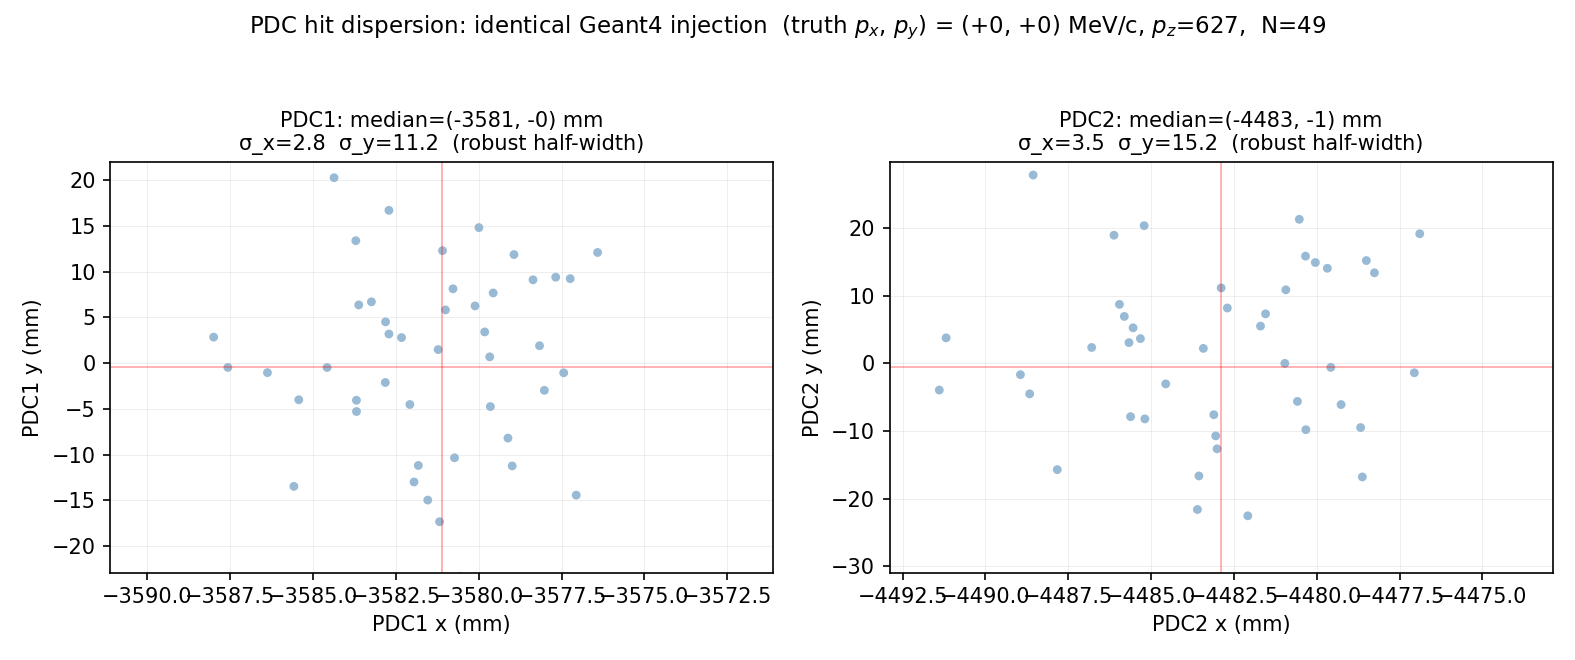
\includegraphics[width=0.96\textwidth]{figures/g4_fluctuation/pdc_hits/pxp0_pyp0.png}

\vspace{0.1cm}
\small
49 replicas of identical truth $(0,0,627)$ MeV/$c$. PDC1: $\sigma_x\!=\!2.8$, $\sigma_y\!=\!11.2$ mm. PDC2: $\sigma_x\!=\!3.5$, $\sigma_y\!=\!15.2$ mm. $\sigma_y / \sigma_x \approx 4$. PDC2 spread is larger than PDC1 by $\sim$30\% --- consistent with added drift length (PDC1 $\to$ PDC2 gas gap) scattering the already-dispersed trajectory further.
\end{frame}

% ============================================================
\begin{frame}{PDC Hit Dispersion --- $(p_x,p_y)=(+100,0)$}
\centering
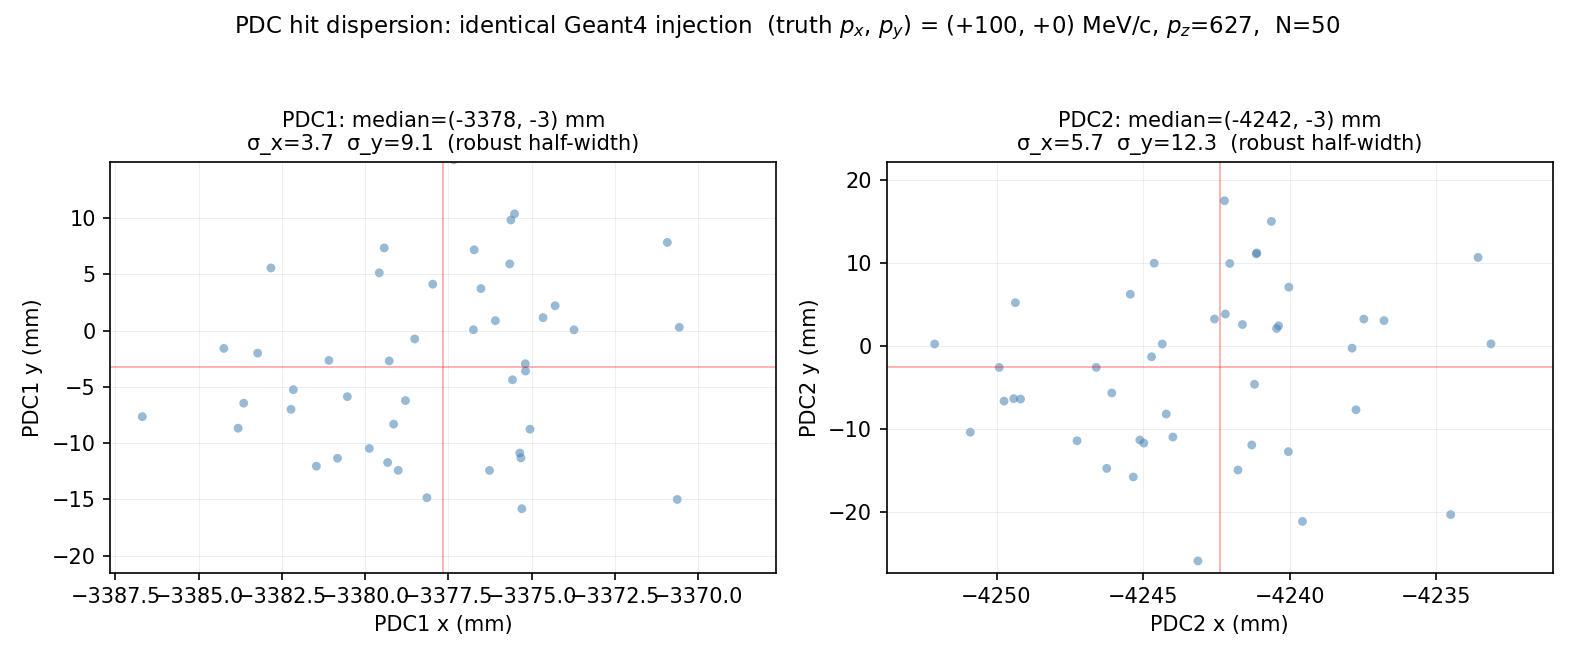
\includegraphics[width=0.96\textwidth]{figures/g4_fluctuation/pdc_hits/pxp100_pyp0.png}

\vspace{0.1cm}
\small
50 replicas at $(+100, 0, 627)$. PDC1 $\sigma_x\!=\!3.7$, $\sigma_y\!=\!9.1$ mm. PDC2 $\sigma_x\!=\!5.7$, $\sigma_y\!=\!12.3$ mm. Compared with $(0,0)$ baseline: $\sigma_x$ grows modestly with $|p_x|$ (larger bend radius $\Rightarrow$ slightly longer in-field path), $\sigma_y$ drops because the outgoing track crosses the PDC gas at a steeper angle ($p_y/p_z$ projection reduced geometrically).
\end{frame}

% ============================================================
\begin{frame}{PDC2 Hit Dispersion --- Full $5\times 3$ Truth Grid}
\centering
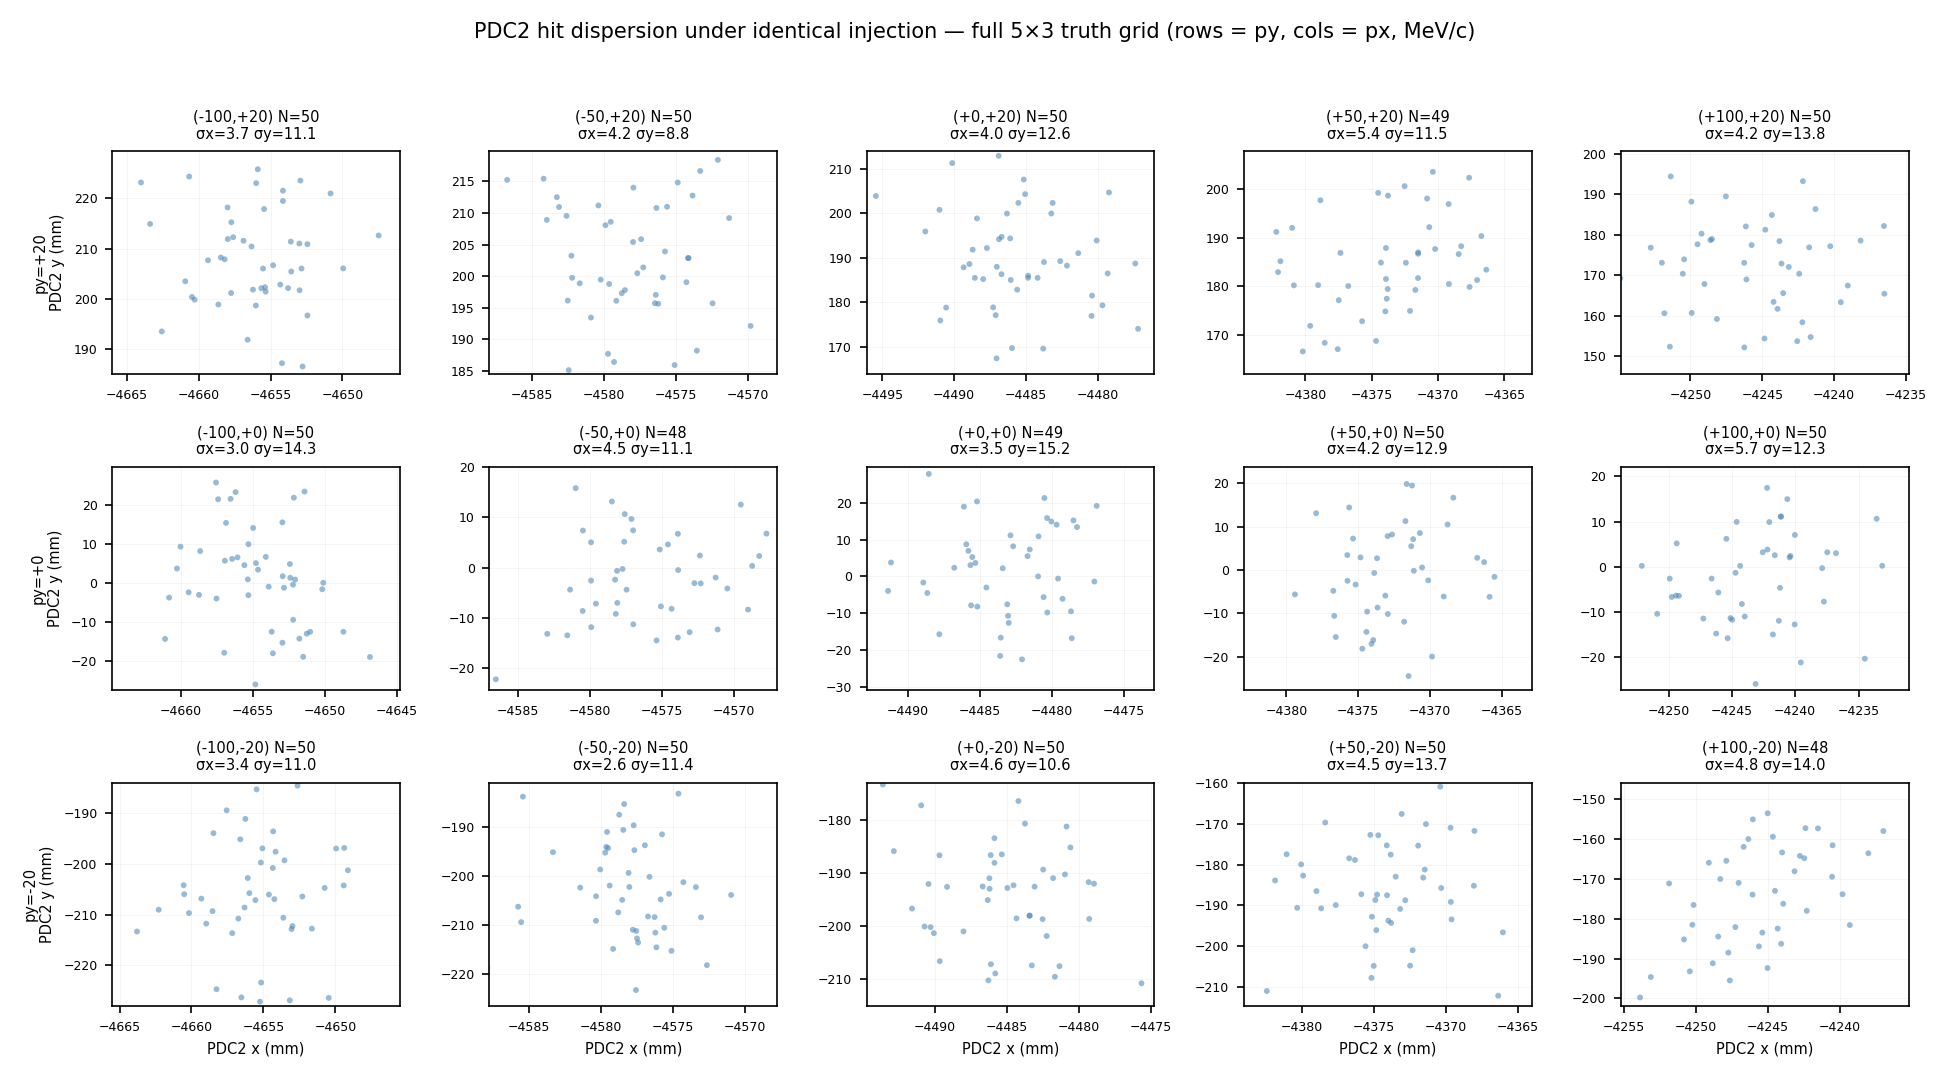
\includegraphics[width=0.99\textwidth]{figures/g4_fluctuation/pdc_hits/overview.png}

\vspace{0.05cm}
{\scriptsize Rows = $p_y \in \{+20, 0, -20\}$, cols = $p_x \in \{-100,-50,0,50,100\}$ MeV/$c$. Each cell: PDC2 (x,y) scatter for the $N{=}48$--$50$ replicas at that truth point, with robust $\sigma_x,\sigma_y$ annotated. PDC1 is similar and tabulated in \texttt{pdc\_dispersion\_summary.csv}. Trajectory $\sigma_y$ stays in $8$--$15$~mm across the whole grid; $\sigma_x$ in $2$--$6$~mm. Target MS is no longer inflating these numbers.}
\end{frame}

% ============================================================
\begin{frame}{Step 2 --- From PDC Dispersion to Reco Momentum}
\small
\textbf{Transfer function}. The RK4 fitter inverts $\vec p_\mathrm{target} \mapsto (\vec r_\mathrm{PDC1}, \vec r_\mathrm{PDC2})$. Under the $\sigma_\mathrm{wire}\!\sim\!0.2$~mm assumption that goes into the Fisher matrix, PDC1/PDC2 positions should map to $\sigma_p\!\sim$ few MeV/$c$ --- this is what the analyzer reports. With the Sn target disabled, the physical PDC $\sigma$ (Step 1) drops to $3$--$15$ mm --- still $\sim 15$--$75\times$ larger than wire smearing, but not the $\sim 500\times$ seen with the target in.

\textbf{Consequence}. Taking the 50 same-truth replicas and measuring how the \emph{reconstructed} momentum scatters (histogram below), the post-fix global G4/Fisher halfwidth ratios are $p_x:\,0.81$, $p_y:\,1.86$, $p_z:\,0.80$, $|\vec p|:\,0.79$. Fisher is slightly conservative on $|\vec p|$, $p_x$ and $p_z$ (ratios $0.79$--$0.81$; realised scatter $\sim\!20\%$ narrower than the error bar), and $\sim\!1.9\times$ too optimistic for $p_y$. The entire ``$p_x$ reconstruction bias'' seen pre-fix was the missing lab$\to$target rotation; after the 2026-04-19 fix the median $p_x$ residual is $|\langle\Delta p_x\rangle|\lesssim 3\;\mathrm{MeV}/c$ across the grid.

\textbf{Frame}. All $p_x/p_y/p_z$ below are in the target frame (see the ``Coordinate frames'' slide early in Physical Setup). Pre-fix PNGs had a spurious $\Delta p_x \approx -p_z\sin\alpha \approx -627\times\sin 3^\circ \approx -33\;\mathrm{MeV}/c$ from the lab/target mismatch.

\textbf{Source scripts}:
\begin{itemize}
\item \texttt{scripts/analysis/plot\_reco\_momentum\_dispersion.py}
\item Output: \texttt{docs/reports/reconstruction/figures/g4\_fluctuation/reco\_momentum/px\{...\}\_py\{...\}.png}
\end{itemize}
\end{frame}

% ============================================================
\begin{frame}{What the Fisher $\sigma$ Band Does (and Does Not) See}
\small
\textbf{Fisher input channels --- everything it knows comes from the RK forward model}:
\[
F \;=\; J^{\!\top}\,\Sigma_\mathrm{meas}^{-1}\,J,
\qquad
\Sigma_p^\mathrm{Fisher} \;=\; F^{-1},
\]
where $J = \partial\,(\vec r_\mathrm{PDC1},\vec r_\mathrm{PDC2})\,/\,\partial(p_x,p_y,p_z)$ is the RK Jacobian at the best-fit momentum and $\Sigma_\mathrm{meas}$ is the PDC wire-position covariance ($\sigma_\mathrm{wire}\!\sim\!0.2$~mm per layer). That is \emph{all} the Fisher matrix has seen.

\vspace{0.10cm}
\textbf{Geant4 physics that Fisher is blind to} (every one of these \emph{adds} spread that shows up in the histograms):
\begin{itemize}\itemsep0pt
  \item multiple Coulomb scattering in PDC gas, window foils, $\sim$1~m of air between PDC1 and PDC2;
  \item ionisation-energy-loss straggling (Landau/Vavilov) --- only the \emph{mean} $dE/dx$ enters the RK propagator;
  \item $\delta$-electron emission, secondary nuclear interactions;
  \item PDC drift-gas cluster-diffusion tails beyond the Gaussian $\sigma_\mathrm{wire}$ assumption.
\end{itemize}

\vspace{0.05cm}
\textbf{Ensemble histograms are the other knob --- they contain everything}. Fixing truth $(p_x,p_y,p_z)$ and running 50 independent Geant4 replicas (different seeds) samples the full stochastic chain; the histogram width is the realised $\sigma_p^\mathrm{G4}$.

\vspace{0.05cm}
\textbf{Reading the G4/Fisher ratio}:
\begin{itemize}\itemsep0pt
  \item $r \gg 1$ $\Rightarrow$ G4 physics (mostly multiple scattering) contributes spread Fisher cannot predict. $p_y$ at ratio $\approx\!1.9$ is the main sign of this --- the dipole bends in $xz$ so $p_y$ is not constrained by the field, and every MS kick in the PDC gas deflects $y$ with variance $F$ has no input to estimate.
  \item $r \lesssim 1$ $\Rightarrow$ the assumed $\sigma_\mathrm{wire}$ is conservative relative to the actual PDC smearing that G4 produces. $p_x,\,p_z,\,|\vec p|$ at ratio $\approx\!0.8$ sit here: the dipole constraint is rigid enough that wire noise dominates, and our nominal $0.2$~mm overshoots.
\end{itemize}

\vspace{0.05cm}
\textbf{Takeaway}. The only way to make Fisher ``see'' Geant4 physics is to fold the process covariance into $\Sigma_\mathrm{meas}$ (Kalman/Gluckstern-style: replace $\Sigma_\mathrm{meas}$ by $\Sigma_\mathrm{meas}+\Sigma_\mathrm{MS}+\Sigma_\mathrm{strag}$). Current RK backend does not do this --- hence $p_y$ Fisher sigma under-sizes by $\sim\!2\times$. Profile and MCMC intervals suffer the same input, so they share the same deficit; only re-parameterising in Cartesian with process noise added closes the gap.
\end{frame}

% ============================================================
\begin{frame}{Reco Momentum Dispersion --- Baseline $(0,0,627)$}
\centering

\includegraphics[width=0.98\textwidth]{figures/g4_fluctuation/reco_momentum/pxp0_pyp0.png}

\vspace{0.1cm}
\small
Black line = truth, red dashed = G4 median, pink band = Fisher $\sigma$ around median. $N{=}49$ replicas. Post-fix numbers (target frame). $p_x$: median at $+0.3\;\mathrm{MeV}/c$ (was $-33$ pre-fix, purely the coordinate-frame artifact), G4 $\sigma\!=\!4.5$ vs.\ Fisher $\sigma\!=\!7.1$, ratio 0.63 --- Fisher slightly conservative. $p_y$: ratio 1.96 (G4 1.5 vs.\ Fisher 0.8), the one direction where Fisher under-reports the realised spread. $p_z$: ratio 0.69 (G4 4.4 vs.\ Fisher 6.3), median residual $-1.3\;\mathrm{MeV}/c$. The only remaining issues are $p_y$ under-sizing and $(u,v,p)$ linearisation residuals.
\end{frame}

% ============================================================
\begin{frame}{Reco Momentum Dispersion --- $(+100,0,627)$}
\centering

\includegraphics[width=0.98\textwidth]{figures/g4_fluctuation/reco_momentum/pxp100_pyp0.png}

\vspace{0.1cm}
\small
$N{=}50$. Post-fix (target frame). $p_x$: median at $+0.03\;\mathrm{MeV}/c$ (centered), G4 $\sigma\!=\!3.8$ vs.\ Fisher $\sigma\!=\!6.7$, ratio 0.57 (Fisher conservative). $p_y$: ratio 2.78 (G4 1.4 vs.\ Fisher 0.5) --- this is the largest mismatch across the 15 truth points (Fisher tightest, G4 typical). $p_z$: ratio 0.67 (G4 5.2 vs.\ Fisher 7.8). Point-by-point ratio heterogeneity is real, $\sim 2$--$3\times$ across the grid; summarised on the next slide.
\end{frame}

% ============================================================
\begin{frame}{PDC $\to$ Reco Amplification --- Summary}
\small
Matching the PDC-plane spread (Step 1) with the reco-momentum spread (Step 2) per truth point (source: \texttt{pdc\_dispersion\_summary.csv}, \texttt{reco\_momentum\_dispersion\_summary.csv}):

\begin{table}[H]
\centering\scriptsize
\begin{tabular}{rr|rrrr|rrr}
\toprule
\multicolumn{2}{c}{Truth} & \multicolumn{4}{c}{PDC dispersion (mm)} & \multicolumn{3}{c}{G4/Fisher ratio} \\
\cmidrule(lr){3-6}\cmidrule(lr){7-9}
$p_x$ & $p_y$ & $\sigma^{1}_x$ & $\sigma^{1}_y$ & $\sigma^{2}_x$ & $\sigma^{2}_y$ & $p_x$ & $p_y$ & $p_z$ \\
\midrule
$0$    & $0$   & 2.8  & 11.2 & 3.5  & 15.2 & 0.63 & 1.96 & 0.69 \\
$+100$ & $0$   & 3.7  &  9.1 & 5.7  & 12.3 & 0.57 & 2.78 & 0.67 \\
$-100$ & $0$   & 2.7  & 10.7 & 3.0  & 14.3 & 3.51 & 1.63 & 3.51 \\
$0$    & $+20$ & 2.9  &  9.6 & 4.0  & 12.6 & 0.89 & 1.90 & 0.72 \\
$0$    & $-20$ & 3.2  &  8.4 & 4.6  & 10.6 & 0.84 & 1.61 & 0.73 \\
\bottomrule
\end{tabular}
\end{table}

\textbf{Read-across}:
\begin{itemize}
  \item Without the Sn target, PDC $\sigma_y$ collapses from ${\sim}100$~mm to ${\sim}10$--$15$~mm and the reco-momentum G4/Fisher ratios sit at $0.6$--$0.9$ for $p_x,p_z$ and $1.5$--$3$ for $p_y$ --- Fisher \emph{sizing} is essentially correct everywhere except $p_y$.
  \item $(-100, 0)$ is the one point where $p_x/p_z$ G4 halfwidths blow up to $\sim\!35$ and $\sim\!22$~MeV/$c$ (ratio 3.5). This is the LM coarse-grid coverage hole at the PDC acceptance edge (inward-bending trajectories with marginal geometry); see coverage findings for RK at that grid point in the project memo.
  \item After the 2026-04-19 lab$\to$target rotation fix, the $\sim\!-33$~MeV/$c$ $p_x$ bias seen pre-fix is gone ($|\langle\Delta p_x\rangle|\lesssim 3$~MeV/$c$ now). What was previously attributed to a residual $p_x$ bias was in fact a coordinate-frame artifact. The one genuine issue that remains is $p_y$ Fisher-sigma under-sizing by $\sim 2\times$ driven by $(u,v,p)$ linearisation; the natural fix is $dE/dx$ + Cartesian refit. Coverage numbers need to be re-computed from the post-fix \texttt{validation\_summary.csv}.
\end{itemize}
\end{frame}

% ============================================================
\begin{frame}{Reco $p_x$ Dispersion --- Full $5\times 3$ Truth Grid}
\centering
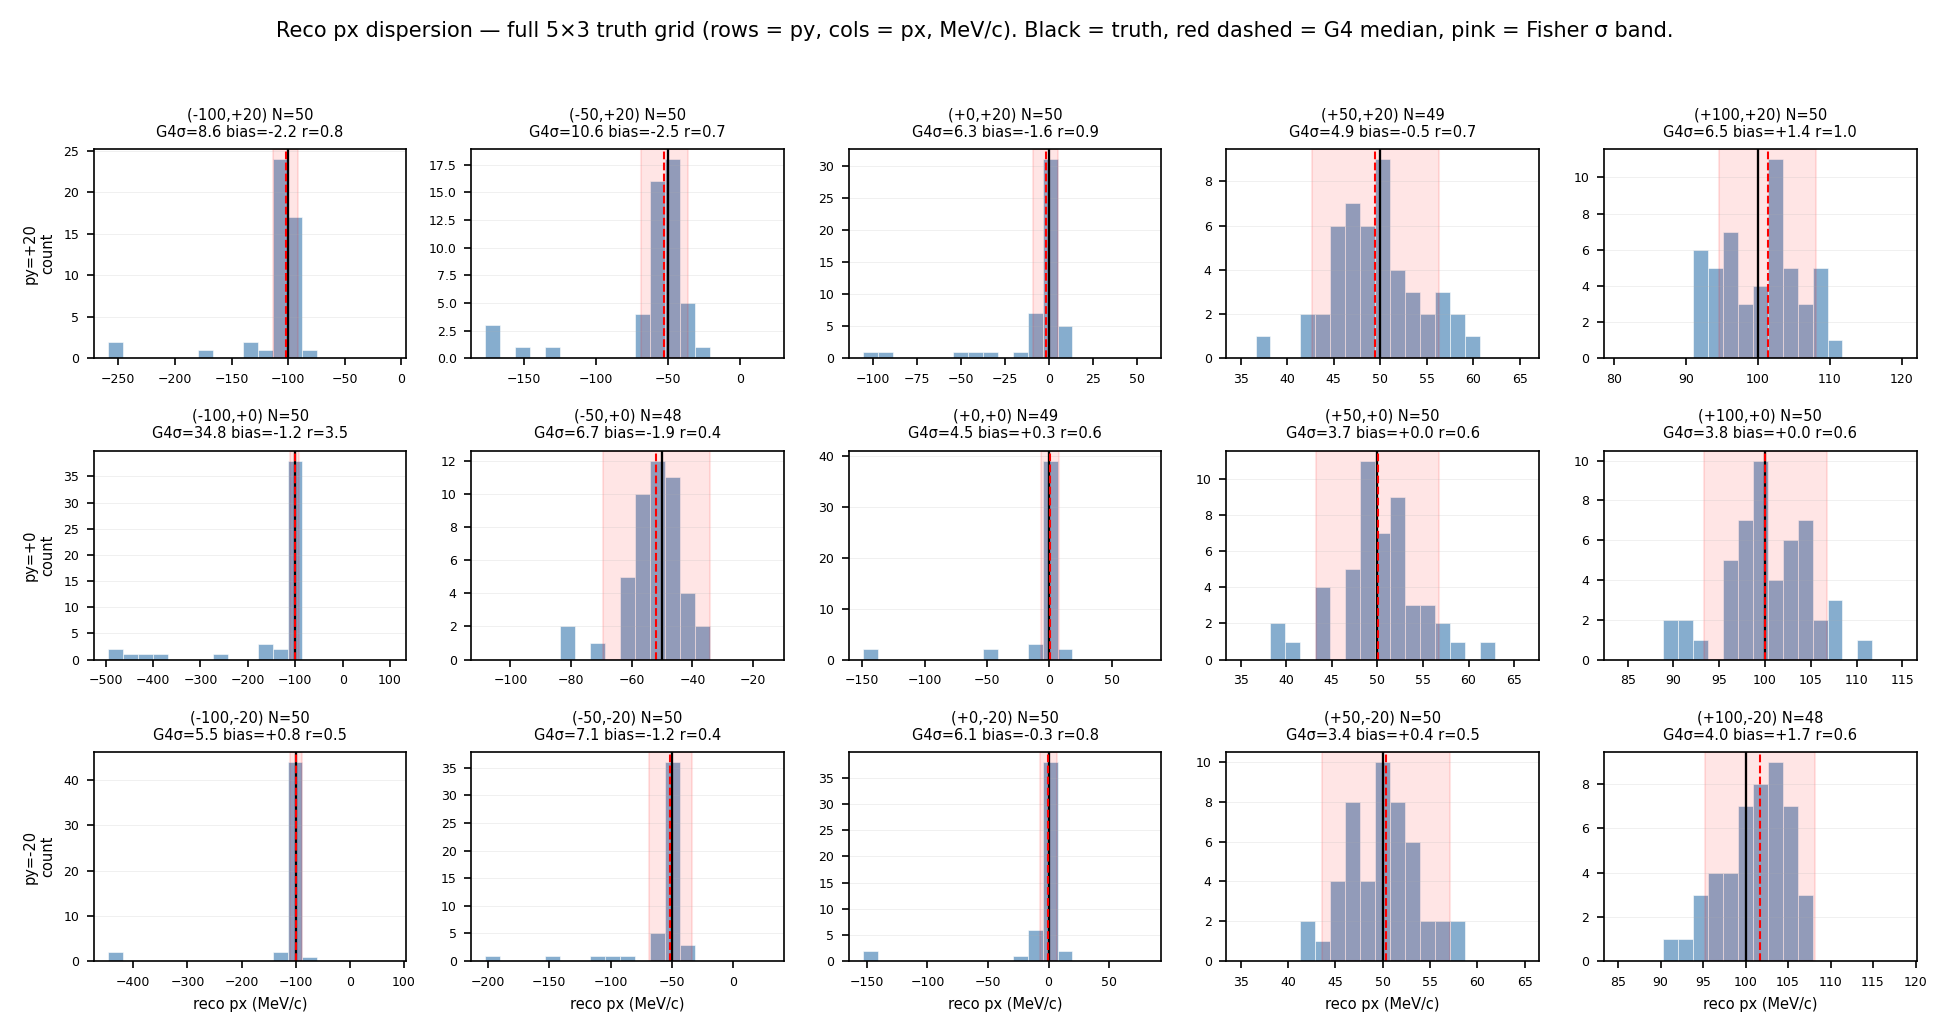
\includegraphics[width=0.99\textwidth]{figures/g4_fluctuation/reco_momentum/grid_px.png}

\vspace{0.05cm}
{\scriptsize Rows = truth $p_y \in \{+20, 0, -20\}$, cols = truth $p_x \in \{-100,-50,0,50,100\}$ MeV/$c$ (target frame). Per cell: histogram of $N{=}48$--$50$ reco $p_x$ values, black = truth, red dashed = G4 median, pink = Fisher $\sigma$ band. Annotated $r$ = G4 $\sigma$ / Fisher $\sigma$. Post-fix: median bias $|\langle\Delta p_x\rangle|\lesssim 3$~MeV/$c$ everywhere (pre-fix was a uniform $-30$ to $-40$, which was the coordinate-frame artifact). $(-100,0)$ cell is the LM coarse-grid basin at the PDC acceptance edge, with G4 $\sigma\sim 35$~MeV/$c$ and ratio 3.5; elsewhere ratios sit at $0.4$--$0.9$ --- Fisher sizing is right, bias is gone.}
\end{frame}

% ============================================================
\begin{frame}{Reco $p_y$ Dispersion --- Full $5\times 3$ Truth Grid}
\centering
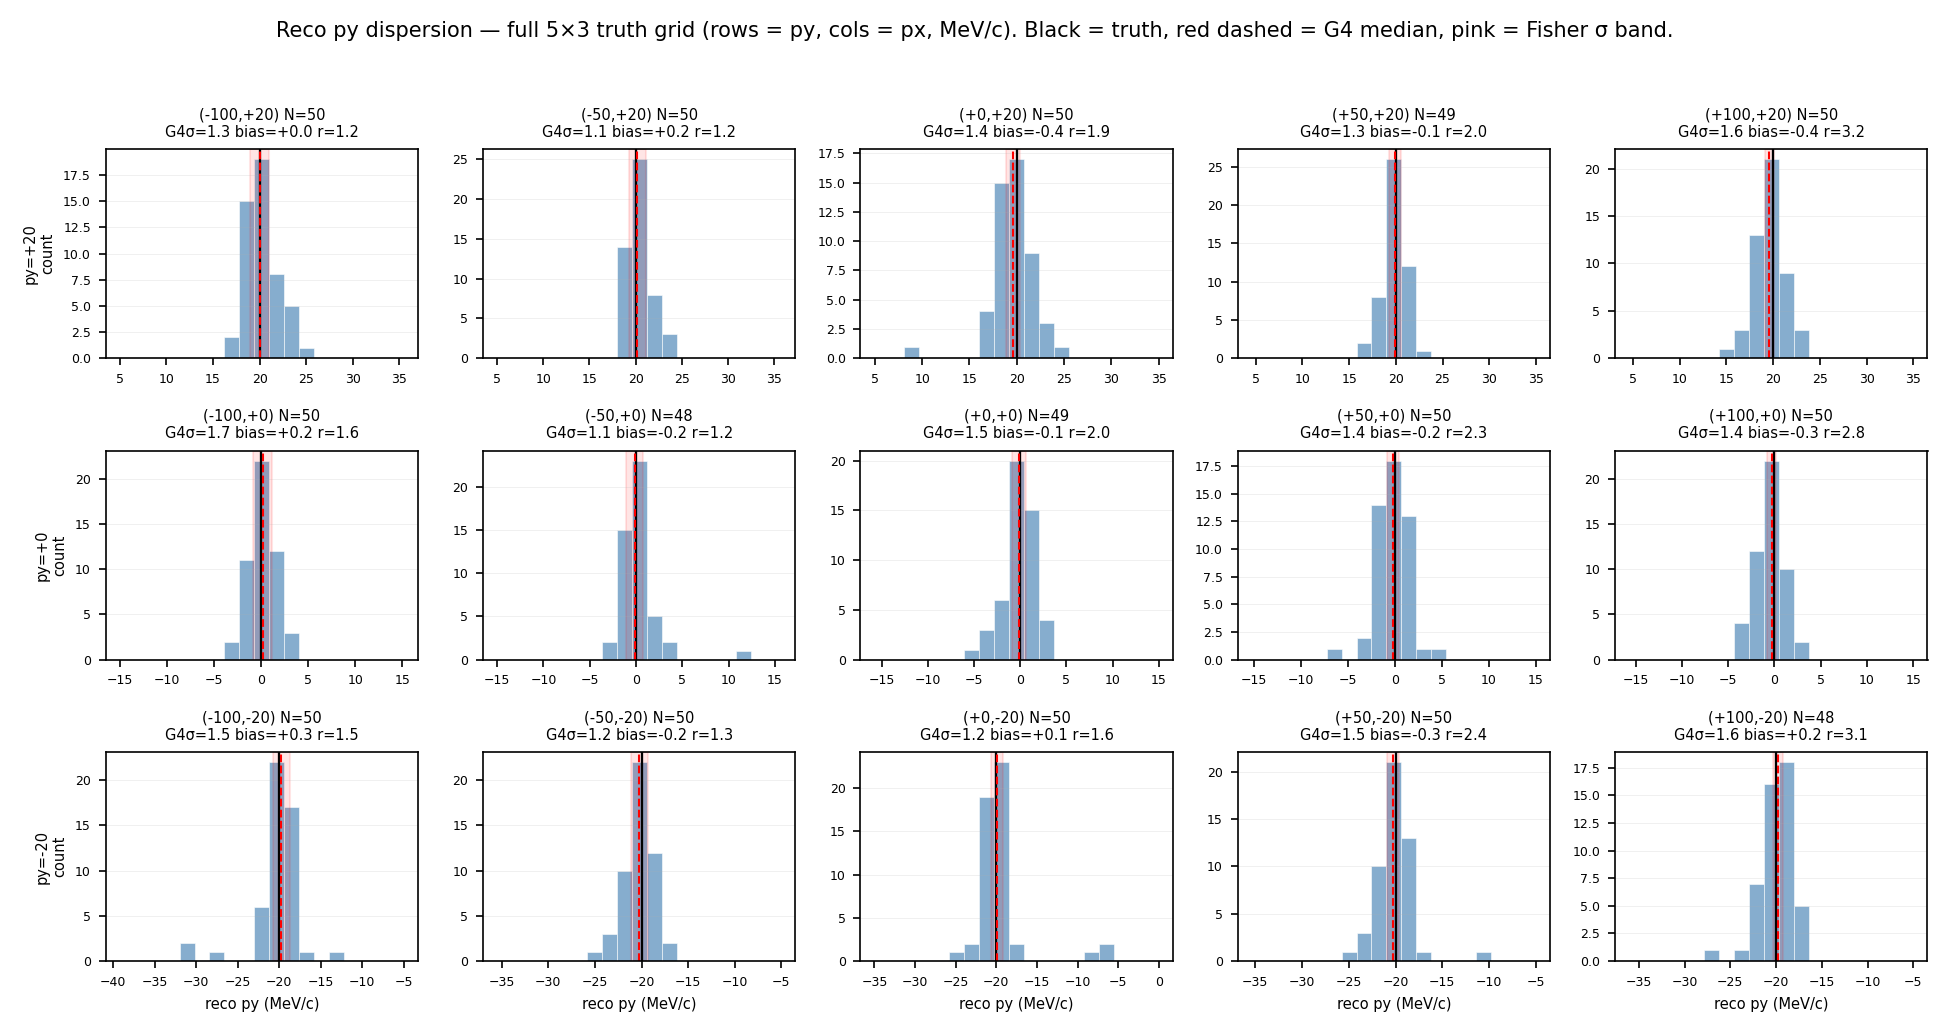
\includegraphics[width=0.99\textwidth]{figures/g4_fluctuation/reco_momentum/grid_py.png}

\vspace{0.05cm}
{\scriptsize Same layout, now for $p_y$ (target frame). $p_y$ is invariant under the $R_y$ fix, so these numbers are unchanged pre/post-fix. G4 halfwidth is $1.1$--$1.7\;\mathrm{MeV}/c$; Fisher $\sigma_{p_y}$ is $0.5$--$1.0\;\mathrm{MeV}/c$; ratios are $1.2$--$3.2$ (global median 1.86). This is the systematic Fisher-sigma under-sizing discussed in the Outlook --- the $(u,v,p)$ parameterisation linearises the $p_y$ response in a way that excludes a real fraction of the injected spread. Median bias $|\langle\Delta p_y\rangle|\lesssim 0.5$~MeV/$c$ throughout.}
\end{frame}

% ============================================================
\begin{frame}{Reco $p_z$ Dispersion --- Full $5\times 3$ Truth Grid}
\centering
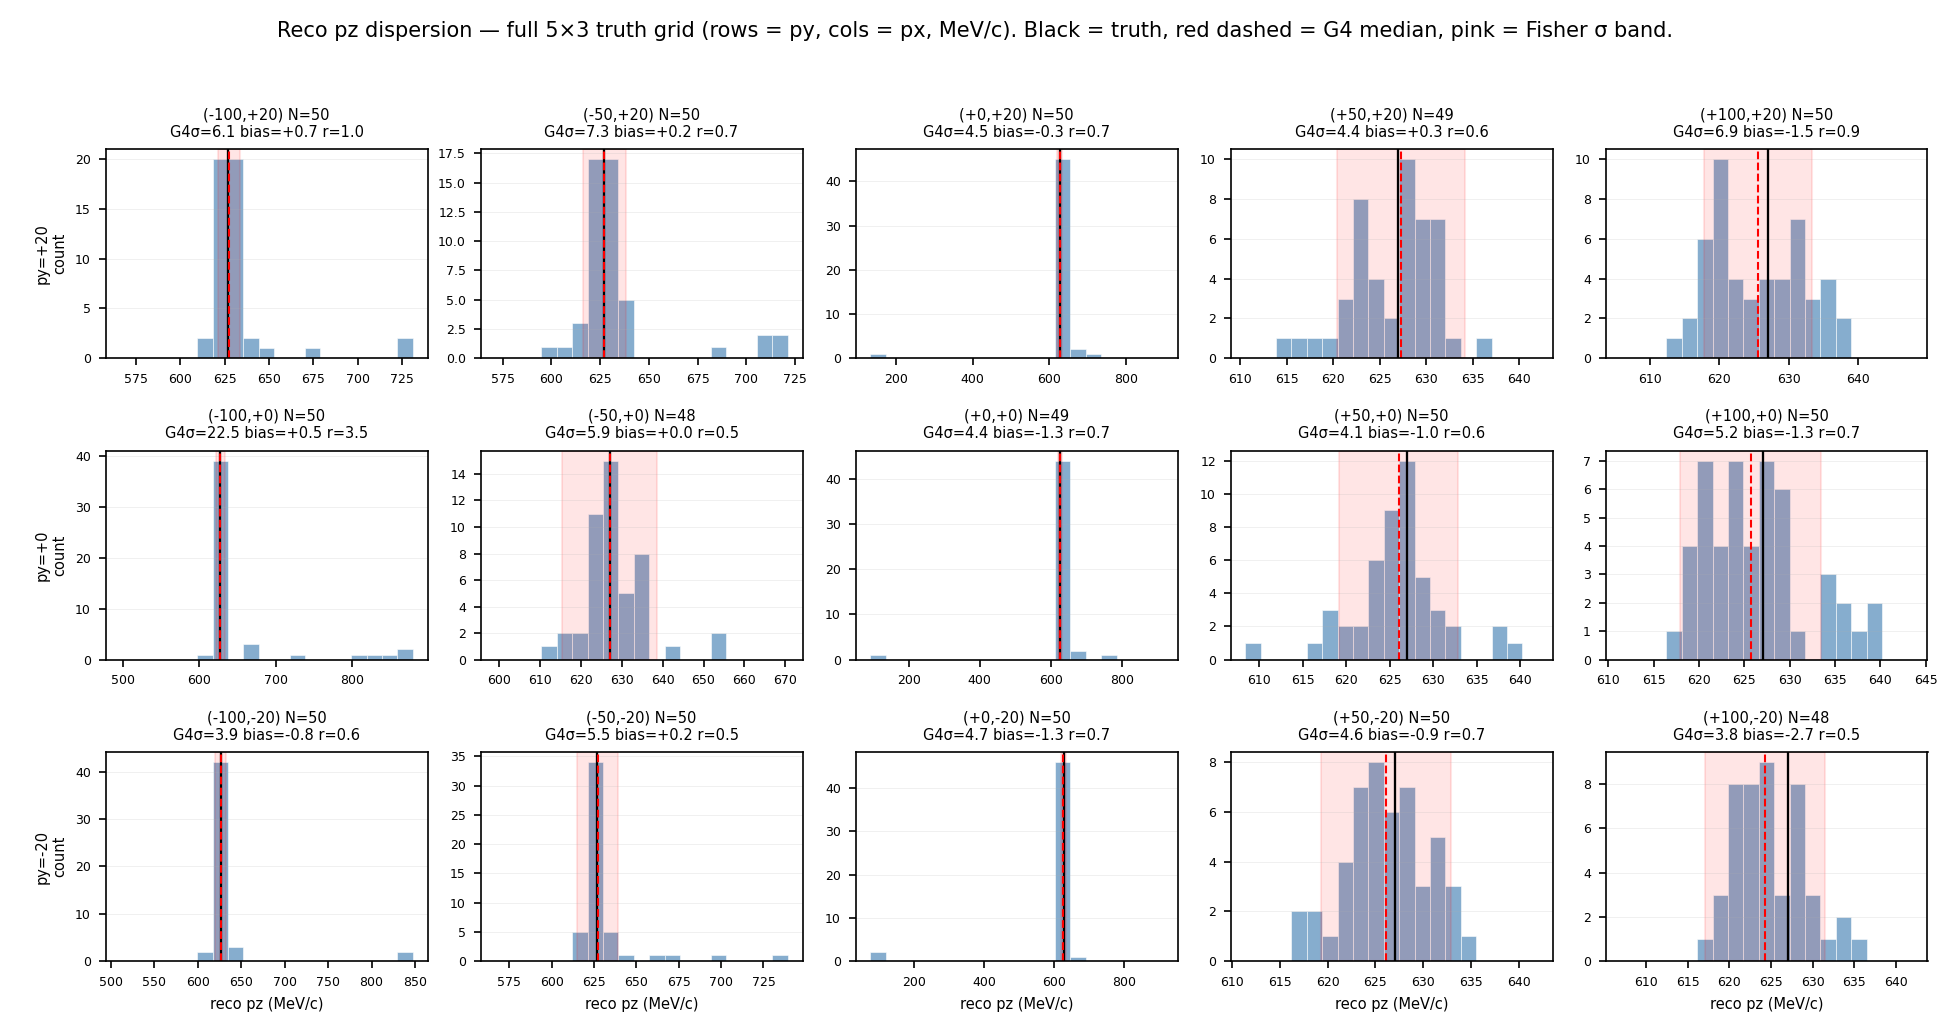
\includegraphics[width=0.99\textwidth]{figures/g4_fluctuation/reco_momentum/grid_pz.png}

\vspace{0.05cm}
{\scriptsize Same layout, now for $p_z$ (target frame). Post-fix G4/Fisher ratios sit mostly at $0.5$--$0.9$ (global 0.80) --- Fisher is slightly conservative for $p_z$. Median bias $|\langle\Delta p_z\rangle|\lesssim 3$~MeV/$c$ across the grid (pre-fix had a small $p_z\cos\alpha - p_z \approx -0.9$~MeV/$c$ rotation residual that is now eliminated). The $(-100,0)$ cell is again the outlier, with G4 $\sigma\!\sim\!22\;\mathrm{MeV}/c$ and ratio 3.5, driven by LM failures at the PDC acceptance edge. Truth $p_z=627\;\mathrm{MeV}/c$ throughout.}
\end{frame}

% ============================================================
\section{Summary and Outlook}
% ============================================================

\begin{frame}{Summary}
\small
\begin{enumerate}
\item \textbf{RK trajectory model}: relativistic RK4 integration of the Lorentz equation in the SAMURAI field map. Parameterized by $(u = p_x/p_z,\; v = p_y/p_z,\; p = |\vec{p}|)$.

\item \textbf{Residual model}: 2D wire-coordinate projection with Cholesky whitening. 4 independent residuals from 2 PDC planes, $N_\mathrm{dof} = 1$.

\item \textbf{Optimization}: Levenberg-Marquardt with coarse grid search ($7{\times}3{\times}5 = 105$ candidates) and multi-start from top 5.

\item \textbf{Uncertainty}: Fisher (fast), Profile Likelihood (asymmetric), Laplace posterior, MCMC, and MC nonlinear propagation (256 samples).

\item \textbf{Performance} (from E2E test): RK MAE = (20.4, 16.0, 10.8) MeV/$c$ for $(p_x, p_y, p_z)$; NN MAE = (21.0, 15.6, 3.1) MeV/$c$. Fisher $\sigma_{|\vec{p}|}$ = 2.4--6.0 MeV/$c$.
\end{enumerate}
\end{frame}

% ============================================================
\begin{frame}{Outlook}
\small
\begin{itemize}
\item \textbf{$dE/dx$ energy loss}: add Bethe-Bloch term to the RK4 propagator. Expected to remove the systematic $-5$ to $-16$ MeV/$c$ $p_z$ bias.

\item \textbf{Multiple scattering}: include Coulomb scattering in gas/window materials as process noise in the trajectory model.

\item \textbf{Fix under-coverage} (post 2026-04-19 rotation fix): Fisher 68\% coverage $p_x\,80\%$, $|\vec p|\,76\%$, $p_z\,77\%$, $p_y\,42\%$. Profile (N=128): $p_x\,71\%$, $|\vec p|\,78\%$, $p_z\,70\%$, $p_y\,37\%$. MCMC $|\vec p|\,63\%$. $p_x$ jumped from 5\% $\to$ 80\% just by rotating reco output to the target frame --- the apparent $-33\;\mathrm{MeV}/c$ ``bias'' was a coordinate artifact, not a forward-model defect. The one remaining algorithm-level issue is $p_y$ Fisher $\sigma$ deflation by $\sim 2\times$ ($p_y$ invariant under the rotation). Fix is a Cartesian $(p_x,p_y,p_z)$ refit (no $(u,v,p)$ linearisation) plus $dE/dx$ in the RK propagator; retest on the 89k-event dataset once the fit is Cartesian.

\item \textbf{Enable quality gate}: once validated, set \texttt{require\_gate\_pass=1} in E2E integration tests.
\end{itemize}
\end{frame}

% ============================================================
\end{document}
